\documentclass[10pt,a4paper]{report}
\usepackage[utf8]{inputenc}
\usepackage{amsmath}
\usepackage{amsfonts}
\usepackage{amssymb}
\usepackage{ragged2e}
\usepackage{graphicx}
\usepackage{fixltx2e}
\usepackage{multicol}
\usepackage{tabularx}
\usepackage{tikz}
\usetikzlibrary{arrows,shapes,automata,petri,positioning,calc}
\usepackage{hyperref}
\hypersetup{
    colorlinks=true,
    linkcolor=blue,
    filecolor=magenta,      
    urlcolor=blue,
    }
\usepackage{tikz}
\usetikzlibrary{matrix,calc}
\usepackage[margin=0.5in]{geometry}
\providecommand{\norm}[1]{\left\lVert#1\right\rVert}
\newcommand{\myvec}[1]{\ensuremath{\begin{pmatrix}#1\end{pmatrix}}}
\let\vec\mathbf
\newcommand{\mydet}[1]{\ensuremath{\begin{vmatrix}#1\end{vmatrix}}}
\providecommand{\mtx}[1]{\mathbf{#1}}
\newenvironment{Figure}
  {\par\medskip\noindent\minipage{\linewidth}}
  {\endminipage\par\medskip}
\begin{document}
\begin{figure*}[!tbp]
  \centering
  \begin{minipage}[b]{0.4\textwidth}
   
\includegraphics[scale=0.05]{IITH-logo.jpg} 
  \end{minipage}
  \hfill
  \vspace{5mm}\begin{minipage}[b]{0.4\textwidth}
\raggedleft 
\includegraphics[scale=0.6]{nrc.jpeg} 
  \end{minipage}\vspace{0.2cm}
\end{figure*}
\raggedright \textbf{Name}:\hspace{1mm}Syed Tabasum nazeer\hspace{3cm} \Large \textbf{Circle Assignment}\hspace{2cm} % 
\normalsize \textbf{Roll No.} :\hspace{1mm} FWC22093\vspace{1cm}
\begin{multicols}{2}
\raggedright \textbf{Problem Statement:}\vspace{2mm}
\raggedright \\C1 and C2 are two concentric circles, the radius of C2 being twice that of C1. From a point P on C2, a tangent PA and PB are drawn to C1. Prove that the centroid of the triangle PAB lies on C1.
\vspace{5mm}
 \vspace{2mm} \\
 \textbf{Construction:}
\begin{center}
\setlength{\arrayrulewidth}{0.5mm}
\setlength{\tabcolsep}{6pt}
\renewcommand{\arraystretch}{1.5}
    \begin{tabular}{|l|c|} \hline
    \textbf{Parameters} & \textbf{Description} \\ \hline
   r & $Radius $
    \\ \hline
   P & $ External point$ 
   \\ \hline  
   C1,C2 & $ concentric circles$ 
   \\ \hline
      \end{tabular}
  \end{center}
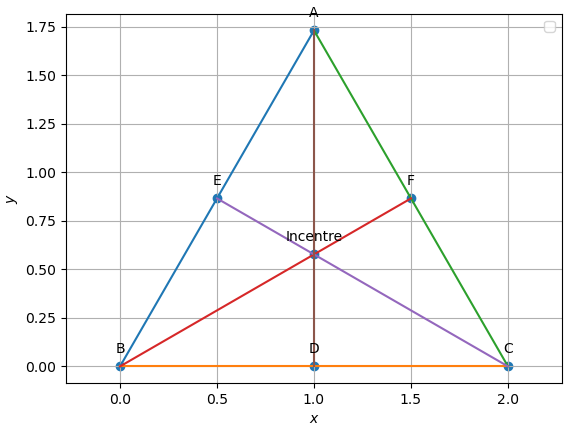
\includegraphics[scale=0.4]{Picture.png}
\\
\textbf{Step1:}\justify{With centre as origin draw two concentric circles with radius r1 and r2 = 2r1 (as per the given condition)}
\\
\textbf{Step2:}\justify{Consider the external point P which is on outer circle. Now the point of contacts of tangents from point P on the inner circle is found by the following equations}
\begin{align}
\boxed{\vec{q}_i = \vec{V^-1}(k_i\vec{n_i-u})}....(i = 1,2) 
\end{align}
\\
\textbf{Step3:} \justify{On solving the above euation, we will obtain four points. Select any two points from consecutive quadrants w.r.t the external point and draw the triangle.}
\\
\textbf{Step4:} \justify{Find the centroid of the triangle using the three points as vertices and plot. The centroid will lie on the inner circle.}
\newline
\\
\textbf{Solution:}
\justify{Let the centre of the concentric circles be 'O' is at origin and the radius of two circles be r1 and r2. As per the condition, r1 and r2 are taken in such a way that r2 = 2r1. Consider a point on the outer circle at (0,r2). Now, to find the point of contact of the two tangents drawn from an external point Q to a circle can be found from the following equation} 
\begin{align}
\boxed{\vec{q}_i = \vec{V^-1}(k_i\vec{n_i-u})}....(i = 1,2) 
\end{align}
Here, 
\begin{align}
k_i = \pm\sqrt{\frac{f_0}{\vec{n^TV^-1n}}}
\end{align}
\begin{align}
f_0 = \vec{u^TV^-1u}-f
\end{align}
\begin{align}
n_1 = \vec{P}\myvec{\sqrt{|\lambda_1|} \\ \sqrt{|\lambda_2|}}
\end{align}
\begin{align}
n_2 = \vec{P}\myvec{\sqrt{|\lambda_1|} \\ -\sqrt{|\lambda_2|}}
\end{align}
\begin{align}
\vec{P} = (\vec{Vh+u})(\vec{Vh+u})^T-\vec{V(h^TVh+2u^Th}+f)
\end{align}
\justify{On solving the above equations, we get two point of contacts of tangents to the inner circle, let it be A,D. As the point P lies on the outer circle, the equation of the circle is given by}
\begin{align}
\vec{x^TVx + 2u^Tx + }f_2 = 0
\end{align}
\justify{Now substitute P in place of x. Here, $\vec{V} = \myvec{1 \ 0 \\ 0 \ 1}$ and $\vec{u} = \myvec{0 \\ 0}$. Then equation (8) becomes}
\begin{align}
\vec{P^TP + }f_2 = 0
\end{align}
\begin{align}
\norm{\vec{P}}^2+f_2 = 0
\end{align}
Let the inner circle equation be 
\begin{align}
\vec{x^TVx + 2u^Tx + }f_1 = 0
\end{align}
As the points A, D lies on the inner circle, equation (11) becomes 
\begin{align}
\vec{A^TA + }f_1 = 0
\end{align}
\begin{align}
\norm{\vec{A}}^2+f_1 = 0
\end{align}
\begin{align}
\vec{D^TD + }f_1 = 0
\end{align}
\begin{align}
\norm{\vec{D}}^2+f_1 = 0
\end{align}
\justify{On solving the equation (13) or equation (15), we get the value of '$f_1$'. Similarly, on solving the equation (10), we get the values of '$f_2$'.}
\newline
Now, the centroid 'C' of the triangle PAB is given by
\begin{align}
\vec{C} = \frac{\vec{P+A+D}}{3}
\end{align}
\textbf{Proof:}
To prove that the centroid of triangle PAD, substitute the point C in the inner circle equation(11)
\begin{align}
\vec{C^TC + }f_1 = 0
\end{align}
\begin{align}
\norm{\vec{C}}^2+f_1 = 0
\end{align}
\justify{The value of '$f_1$' can be found out on solving the equation (13) or equation (14). On  substituting the value of '$f_1$' and norm of C in equation (18). These two values satisfies the equation(18). Therefore, it can be concluded that the centroid of triangle PAD lies on the inner circle.}
\end{multicols}
\end{document}
